\documentclass{article}

% Pacotes
\usepackage[utf8]{inputenc}
\usepackage[brazil]{babel}
\usepackage[letterpaper,top=2.5cm,bottom=2.5cm,left=3cm,right=3cm,marginparwidth=1.75cm]{geometry}
\usepackage{amsmath, graphicx, subcaption}
\usepackage[colorlinks=true, allcolors=blue]{hyperref}

\usepackage{listings}
\usepackage{xcolor}
\usepackage{tabularx}
\usepackage{array}
\usepackage{amssymb}    % símbolos matemáticos extras
\usepackage{url}
\usepackage{booktabs}   % Para top/mid/bottomrule
\usepackage{float}      % Para [H]
\usepackage{enumitem}   % Para customizar listas (a), (b), (c)


% Definições de estilo para Python
\lstdefinestyle{pythonstyle}{
      language=Python,
      basicstyle=\ttfamily\small,
      keywordstyle=\color{blue}\bfseries,
      commentstyle=\color{gray}\itshape,
      stringstyle=\color{orange},
      numbers=left,
      numberstyle=\tiny,
      stepnumber=1,
      numbersep=10pt,
      backgroundcolor=\color{white},
      frame=single,
      breaklines=true,
      tabsize=4,
      showstringspaces=false,
      % Permite acentos e símbolos nos comentários do código
      literate={á}{{\'a}}1 {à}{{\`a}}1 {ã}{{\~a}}1 {â}{{\^a}}1
               {é}{{\'e}}1 {ê}{{\^e}}1 {í}{{\'i}}1 {ó}{{\'o}}1
               {õ}{{\~o}}1 {ô}{{\^o}}1 {ú}{{\'u}}1 {ç}{{\c{c}}}1
               {Á}{{\'A}}1 {É}{{\'E}}1 {Í}{{\'I}}1 {Ó}{{\'O}}1
               {Ú}{{\'U}}1 {Ç}{{\c{C}}}1 {Ã}{{\~A}}1 {º}{{$^{\circ}$}}1,
}

\renewcommand{\lstlistingname}{Listagem}
\setlength{\emergencystretch}{2em} % evita linhas estouradas com trechos de código no texto

\begin{document}

% Capa personalizada
\begin{titlepage}
      \centering
      \IfFileExists{images/fig_logo_cefetmg.pdf}{\includegraphics[width=4cm]{images/fig_logo_cefetmg.pdf}\par}{}
      \vspace{0.5cm}

      {\LARGE Centro Federal de Educação Tecnológica de Minas Gerais \par}
      \vspace{0.2cm}

      {\Large Engenharia de Computação \\ Computação Gráfica \par}
      \vspace{4cm}

      {\Huge \textbf{Relatório de Desenvolvimento} \par}
      \vspace{0.5cm}

      {\LARGE Casa 3D com Shaders e Interpolação de Textura \par}
      \vspace{3cm}

      {\LARGE João Paulo da Cunha Faria \par}
      {\LARGE Maria Eduarda Teixeira Souza \par}
      \vfill

      {\large Divinópolis - MG \par}
      {\large Outubro de 2026 \par}
\end{titlepage}


\section{Introdução}

Na Aula 17 foi apresentado o uso de texturas com \textit{shaders}. Até a aula anterior, cada vértice carregava uma cor fixa, e a única forma de deixar um sólido mais detalhado era acrescentar mais vértices. Com textura, a ideia muda: uma imagem lida do disco é ``colada'' sobre os triângulos, e cada pixel da tela busca a sua cor dentro dessa imagem. Como exemplo, o professor mostrou o programa \texttt{cubo\_textura.py}, que desenha um cubo de pedras que gira com as setas do teclado, usando filtro linear e \textit{mipmaps}.

Ao final da aula foi proposta a seguinte atividade:

\begin{quote}
\textit{Construa uma casa 3D usando apenas cubos/quadrados, pirâmides/triângulos e texturas. Inclua rotações usando as setas do teclado.}
\end{quote}

Para resolver a atividade, foi criado o programa \texttt{casa.py}, que parte do cubo da aula e monta a casa com quatro objetos: o corpo (um cubo), o telhado (uma pirâmide de base quadrada), a porta e as janelas (quadrados colados nas paredes). Cada objeto recebe a sua própria textura. Como as imagens usadas em aula não estavam disponíveis, também foi criado o programa \texttt{gerar\_texturas.py}, que gera as quatro texturas (tijolo, telha, madeira e vidro) com a biblioteca Pillow. Este relatório explica como os dois programas foram construídos e mostra o resultado da execução.

\section{Fundamentação}

\subsection{Textura e Coordenadas UV}\label{sec:uv}

Uma textura é apenas uma imagem guardada na memória da placa de vídeo. Cada pixel dessa imagem é chamado de \textit{texel} (\textit{texture element}), para não ser confundido com os pixels da tela. Para dizer qual parte da imagem vai em qual parte do triângulo, cada vértice recebe, além da posição $(x, y, z)$, um par de coordenadas $(u, v)$, chamadas de coordenadas UV ou coordenadas de textura.

As coordenadas UV são normalizadas: independentemente do tamanho da imagem em pixels, $(0, 0)$ é o canto inferior esquerdo e $(1, 1)$ é o canto superior direito. Assim, o mesmo código funciona com uma imagem de $256\times256$ ou de $4096\times4096$. Para converter uma coordenada UV em uma posição dentro de uma textura de largura $L$ e altura $A$, a GPU calcula:

\begin{equation}\label{eq:uv_texel}
x_{texel} = u \cdot L - 0{,}5, \qquad y_{texel} = v \cdot A - 0{,}5
\end{equation}

\noindent onde o $-0{,}5$ aparece porque o centro do primeiro texel fica em $0{,}5$, e não em $0$.

O mapeamento é feito vértice a vértice. Na face frontal do cubo, por exemplo, os quatro cantos recebem $(0,0)$, $(1,0)$, $(1,1)$ e $(0,1)$, de modo que a imagem inteira cobre a face. No triângulo do telhado, os dois cantos da base recebem $(0,0)$ e $(1,0)$ e a ponta recebe $(0{,}5;\ 1)$, de modo que apenas um triângulo recortado da imagem aparece na face (Figura~\ref{fig:uv}).

\begin{figure}[H]
    \centering
    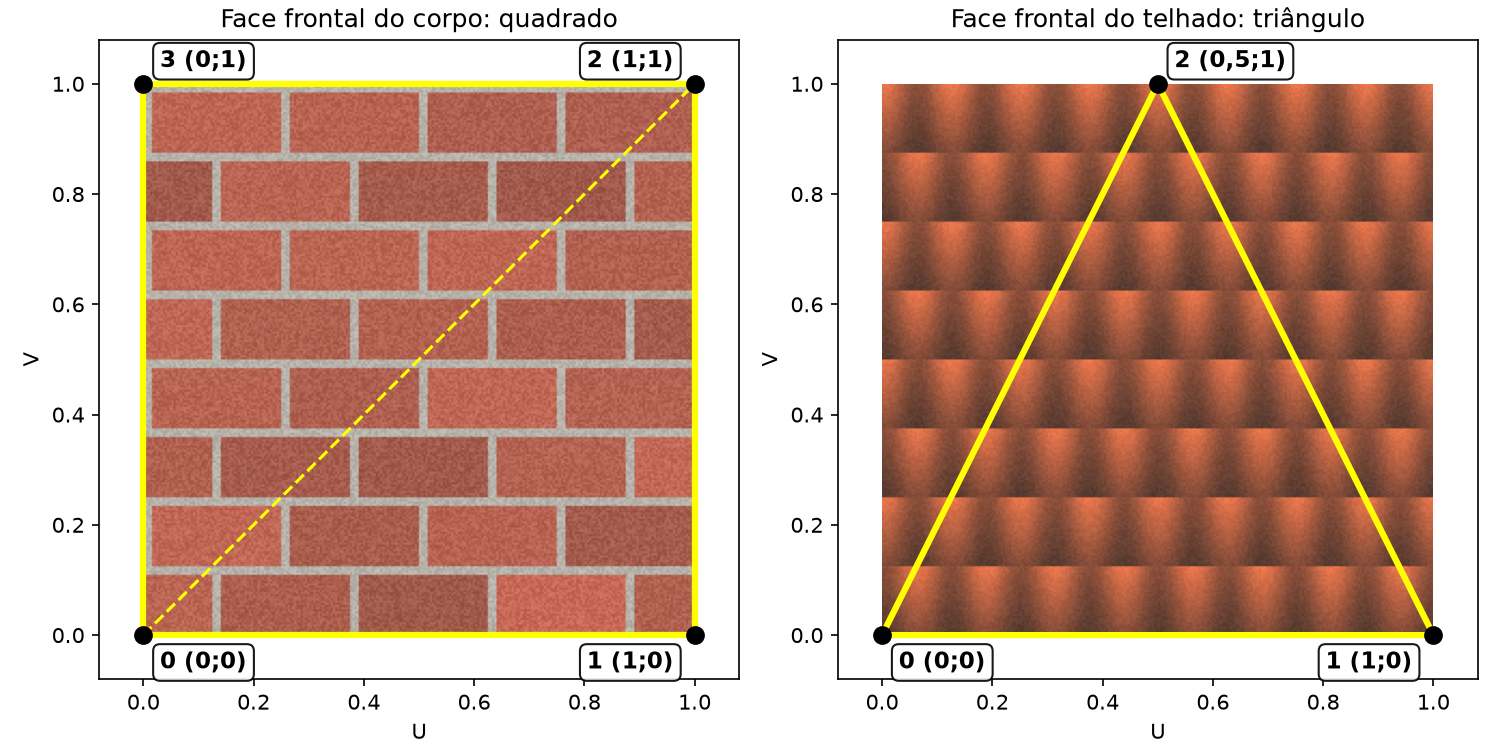
\includegraphics[width=\textwidth]{images/mapeamento_uv.png}
    \caption{Coordenadas UV dos vértices da face frontal do corpo (à esquerda) e da face frontal do telhado (à direita). O número antes do par $(u;v)$ é o índice do vértice dentro da face. A linha tracejada é a diagonal que divide o quadrado em dois triângulos.}
    \label{fig:uv}
\end{figure}

Um detalhe importante é a orientação do eixo $V$. O OpenGL considera que a primeira linha de bytes enviada é a linha de \textbf{baixo} da imagem, mas os arquivos de imagem (PNG, JPG) guardam primeiro a linha de \textbf{cima}. Se a imagem for enviada como está, ela aparece de cabeça para baixo no sólido. Por isso a imagem é invertida verticalmente antes de ser enviada para a GPU.

\subsection{Interpolação das Coordenadas UV}

Os valores de $(u, v)$ só são definidos nos vértices. Para os pixels que ficam no meio do triângulo, o rasterizador da GPU interpola esses valores automaticamente. Um ponto dentro de um triângulo pode ser escrito como uma média ponderada dos três vértices, com pesos $\lambda_0$, $\lambda_1$ e $\lambda_2$ (as coordenadas baricêntricas), que somam 1. A coordenada UV do ponto é obtida com os mesmos pesos:

\begin{equation}\label{eq:baricentrica}
(u, v) = \lambda_0\,(u_0, v_0) + \lambda_1\,(u_1, v_1) + \lambda_2\,(u_2, v_2), \qquad \lambda_0 + \lambda_1 + \lambda_2 = 1
\end{equation}

Na prática, a GPU faz uma versão corrigida dessa equação, que divide cada termo pela coordenada $w$ do vértice (a distância até a câmera, vista na Aula 15). Sem essa correção, a textura ficaria ``torta'' em faces vistas de lado, pois a perspectiva encolhe as partes mais distantes de forma não linear. Nos \textit{shaders}, essa interpolação aparece apenas como uma variável \texttt{out} no \textit{vertex shader} e uma variável \texttt{in} com o mesmo nome no \textit{fragment shader}: o programador não precisa escrever nenhuma conta.

\subsection{Filtros de Textura}\label{sec:filtros}

A coordenada $(x_{texel}, y_{texel})$ da Equação~\ref{eq:uv_texel} quase nunca é um número inteiro, ou seja, ela cai entre texels. O filtro de textura decide qual cor usar nesse caso. O OpenGL tem dois filtros básicos:

\begin{itemize}
    \item \textbf{\texttt{GL\_NEAREST} (vizinho mais próximo):} usa a cor do texel mais próximo. É o mais rápido, mas quando a textura é ampliada cada texel vira um quadrado visível, com aspecto ``pixelado'';
    \item \textbf{\texttt{GL\_LINEAR} (bilinear):} usa os quatro texels vizinhos e faz uma média ponderada pela distância (Figura~\ref{fig:bilinear}).
\end{itemize}

\begin{figure}[H]
    \centering
    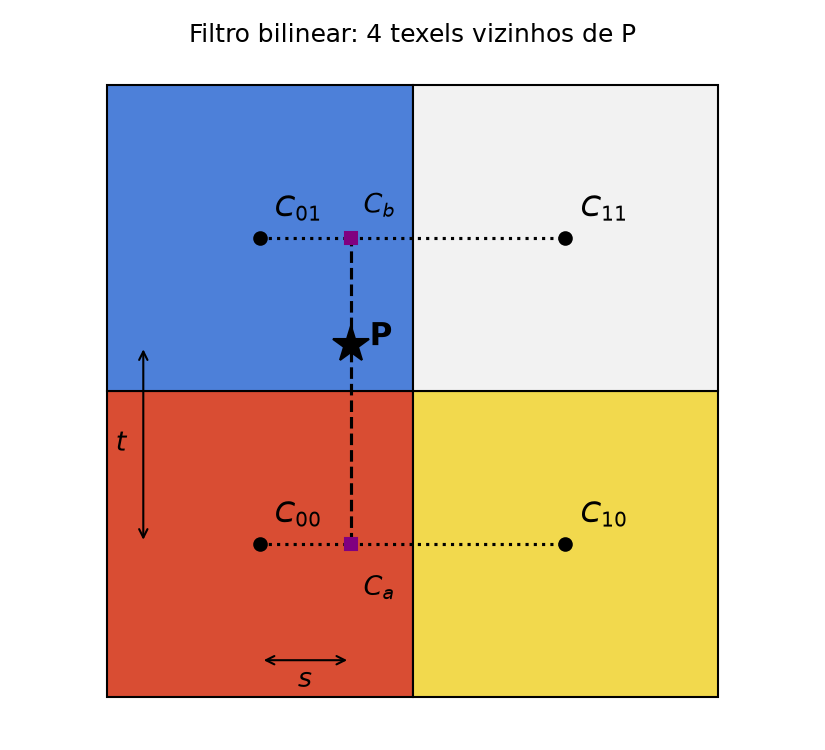
\includegraphics[width=0.5\textwidth]{images/bilinear.png}
    \caption{Filtro bilinear: a cor do ponto P é calculada a partir dos quatro texels vizinhos. Primeiro interpola-se na horizontal ($C_a$ e $C_b$) e depois na vertical.}
    \label{fig:bilinear}
\end{figure}

Sendo $s$ e $t$ as partes fracionárias de $x_{texel}$ e $y_{texel}$, o filtro bilinear faz duas interpolações lineares na horizontal e uma na vertical:

\begin{equation}\label{eq:bilinear}
\begin{aligned}
C_a &= (1 - s)\,C_{00} + s\,C_{10} \\
C_b &= (1 - s)\,C_{01} + s\,C_{11} \\
C_P &= (1 - t)\,C_a + t\,C_b
\end{aligned}
\end{equation}

O filtro é configurado separadamente para duas situações:

\begin{itemize}
    \item \textbf{Ampliação (\texttt{GL\_TEXTURE\_MAG\_FILTER}):} quando a câmera está perto e um texel cobre vários pixels da tela;
    \item \textbf{Redução (\texttt{GL\_TEXTURE\_MIN\_FILTER}):} quando a câmera está longe e vários texels caem dentro de um único pixel.
\end{itemize}

\subsection{Mipmaps}\label{sec:mipmaps}

Na redução, nem o filtro bilinear resolve o problema: se um pixel cobre 20 texels, olhar apenas 4 deles ainda é escolher uma amostra quase aleatória. O resultado é o \textit{aliasing}, um ``serrilhado piscante'' que muda a cada pequeno movimento do objeto.

A solução vista em aula são os \textit{mipmaps}: a função \texttt{glGenerateMipmap} cria cópias da textura cada vez menores, cada uma com metade da largura e da altura da anterior. Para uma textura de $256\times256$, são criados os níveis $128\times128$, $64\times64$, \ldots, até $1\times1$, totalizando 9 níveis. Cada texel de um nível é a média de 4 texels do nível anterior, então os níveis menores já guardam a cor ``média'' de regiões inteiras da imagem. Como $\frac{1}{4} + \frac{1}{16} + \frac{1}{64} + \cdots = \frac{1}{3}$, a pirâmide de \textit{mipmaps} ocupa só um terço a mais de memória.

Durante o desenho, a GPU escolhe o nível cujo texel tem aproximadamente o tamanho de um pixel da tela. Com o filtro \texttt{GL\_LINEAR\_MIPMAP\_LINEAR}, usado neste trabalho, ela faz a interpolação bilinear nos dois níveis mais próximos e depois uma interpolação linear entre eles. Por envolver três interpolações, esse filtro é chamado de \textbf{trilinear}.

\subsection{Repetição da Textura}

Os parâmetros \texttt{GL\_TEXTURE\_WRAP\_S} e \texttt{GL\_TEXTURE\_WRAP\_T} dizem o que fazer quando uma coordenada UV sai do intervalo $[0, 1]$ (no OpenGL, os eixos $U$ e $V$ também são chamados de $S$ e $T$). Com \texttt{GL\_REPEAT}, apenas a parte fracionária é usada: $u = 1{,}3$ é tratado como $u = 0{,}3$, e a imagem se repete como um papel de parede. Neste trabalho todas as coordenadas UV ficam em $[0, 1]$, mas a configuração foi mantida como no exemplo da aula. Ela permite, por exemplo, repetir os tijolos duas vezes em cada parede apenas trocando os valores 1 por 2 nas coordenadas UV, sem precisar de uma imagem maior.

\subsection{A Matriz MVP}

Assim como na Aula 15, cada vértice é levado até a tela pela matriz MVP:

\begin{equation}\label{eq:mvp}
MVP = P \cdot V \cdot M, \qquad M = R_x(\theta_x) \cdot R_y(\theta_y), \qquad V = T(0;\ -0{,}3;\ -4)
\end{equation}

\noindent onde $P$ é a projeção em perspectiva (campo de visão de $45^\circ$, proporção $800/600$, planos de corte em $0{,}1$ e $100$), $V$ afasta a casa 4 unidades da câmera e a desce $0{,}3$ unidade para que o telhado caiba inteiro na janela, e $M$ gira a casa conforme as setas do teclado. As matrizes $T$, $R_x$, $R_y$ e $P$ são as mesmas da Aula 15, então não serão repetidas aqui. O importante para esta atividade é que a \textbf{mesma} MVP é usada para os quatro objetos da casa: como todos foram modelados no mesmo sistema de coordenadas, eles giram juntos, como uma peça só.

\subsection{Geometria da Casa}\label{sec:geometria}

A casa foi modelada com centro do corpo na origem (Figura~\ref{fig:frente}), com quatro objetos:

\begin{itemize}
    \item \textbf{Corpo:} o mesmo cubo da aula, de $-0{,}5$ a $0{,}5$ nos três eixos;
    \item \textbf{Telhado:} uma pirâmide de base quadrada. A base fica em $y = 0{,}5$, apoiada no topo do cubo, e vai de $-0{,}6$ a $0{,}6$ em $x$ e $z$, sendo um pouco maior que o cubo para formar o beiral. O ápice fica em $(0;\ 1{,}1;\ 0)$;
    \item \textbf{Porta:} um retângulo na face frontal, de $x = -0{,}12$ a $0{,}12$ e de $y = -0{,}5$ (chão) a $y = 0{,}1$;
    \item \textbf{Janelas:} quatro quadrados de $0{,}2\times0{,}2$, dois na face frontal (um de cada lado da porta) e um em cada parede lateral.
\end{itemize}

A porta e as janelas não ficam exatamente sobre a parede, mas $0{,}005$ unidade à frente dela (por exemplo, em $z = 0{,}505$ em vez de $z = 0{,}5$). Se ficassem no mesmo plano, a parede e a porta teriam a mesma profundidade em todos os pixels, e o Z-Buffer não teria como decidir qual das duas está na frente. O resultado seria o \textit{z-fighting}: as duas texturas ``brigando'' e piscando conforme a casa gira, devido a pequenos erros de arredondamento. O deslocamento de $0{,}005$ é pequeno demais para ser percebido, mas suficiente para o Z-Buffer.

Como a GPU só desenha triângulos, cada quadrado é dividido em dois triângulos pela diagonal. Além disso, um vértice agora carrega uma coordenada UV, e um mesmo canto do sólido precisa de UVs diferentes em cada face a que pertence. Por isso, cada face tem os seus próprios vértices, e os cantos são repetidos (Tabela~\ref{tab:contagem}).

\begin{table}[H]
\centering
\caption{Quantidade de faces, vértices e triângulos de cada objeto da casa.}
\label{tab:contagem}
\begin{tabular}{llcccc}
\toprule
\textbf{Objeto} & \textbf{Primitiva} & \textbf{Faces} & \textbf{Vértices no VBO} & \textbf{Triângulos} & \textbf{Índices} \\
\midrule
Corpo   & cubo                  & 6 & 24 & 12 & 36 \\
Telhado & pirâmide              & 5 & 16 & 6  & 18 \\
Porta   & quadrado (retângulo)  & 1 & 4  & 2  & 6  \\
Janelas & 4 quadrados           & 4 & 16 & 8  & 24 \\
\midrule
\textbf{Total} &                & 16 & 60 & 28 & 84 \\
\bottomrule
\end{tabular}
\end{table}

\section{Metodologia}

O código está nos arquivos \texttt{casa.py} e \texttt{gerar\_texturas.py}. Nesta seção, os dois são apresentados por inteiro, na ordem em que aparecem nos arquivos, e cada parte é explicada logo após a sua listagem. A numeração das linhas nas listagens é a mesma dos arquivos originais.

\subsection{Materiais e Configuração}

O código foi desenvolvido em \textit{Python} com quatro bibliotecas: \texttt{glfw}, para criar a janela e ler o teclado; \texttt{PyOpenGL}, para enviar os dados e os comandos de desenho para a placa de vídeo; \texttt{NumPy}, para montar as matrizes e os vetores de vértices; e \texttt{Pillow}, para ler e gerar os arquivos de imagem. A instalação é feita com:

\begin{lstlisting}[style=pythonstyle, numbers=none]
pip install glfw PyOpenGL numpy Pillow
\end{lstlisting}

Para executar, primeiro são geradas as texturas e depois é aberta a casa:

\begin{lstlisting}[style=pythonstyle, numbers=none]
python gerar_texturas.py
python casa.py
\end{lstlisting}

\subsection{Geração das Texturas}

O programa \texttt{gerar\_texturas.py} desenha as quatro texturas usadas na casa e as salva na pasta \texttt{texturas/}, ao lado do script (Figura~\ref{fig:texturas}). Todas têm $256\times256$ pixels. Usar uma potência de 2 não é obrigatório no OpenGL 3.3, mas facilita a geração dos \textit{mipmaps}, pois cada nível tem exatamente a metade do tamanho do anterior.

\begin{figure}[H]
    \centering
    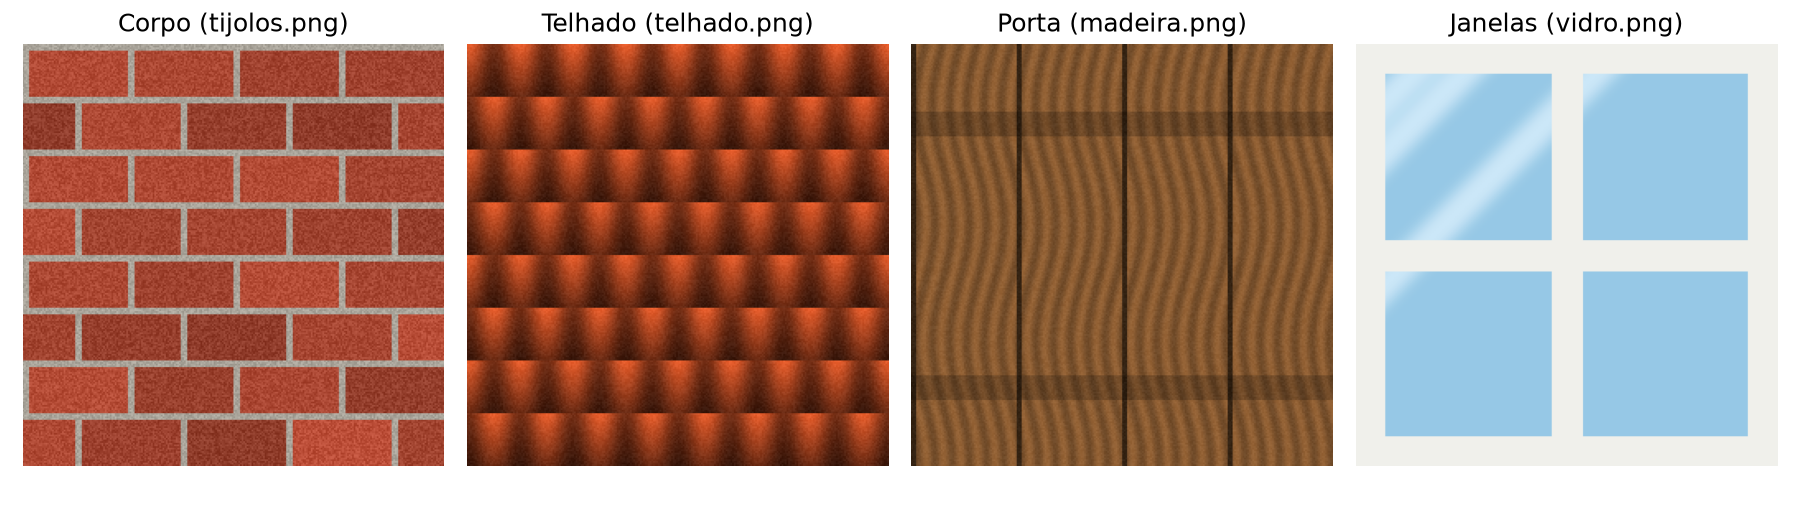
\includegraphics[width=\textwidth]{images/texturas.png}
    \caption{As quatro texturas geradas pelo programa \texttt{gerar\_texturas.py}.}
    \label{fig:texturas}
\end{figure}

O início do arquivo (Listagem~\ref{lst:tex_inicio}) define o tamanho das imagens, a pasta de saída e um gerador de números aleatórios com semente fixa (42), para que as texturas sejam sempre iguais a cada execução. A função \texttt{adicionar\_ruido} soma um valor aleatório entre $-$\texttt{intensidade} e $+$\texttt{intensidade} a cada pixel. O mesmo valor é somado aos três canais (R, G e B), o que deixa o pixel mais claro ou mais escuro sem mudar o tom. Esse ruído imita a textura irregular de materiais reais e evita que as superfícies pareçam ``chapadas''. A função \texttt{np.clip} garante que os valores continuem entre 0 e 255.

\lstinputlisting[style=pythonstyle, firstline=1, lastline=20, firstnumber=1, caption={Importações, constantes e função de ruído}, label={lst:tex_inicio}]{code/gerar_texturas.py}

A textura de tijolos (Listagem~\ref{lst:tex_tijolos}) começa com o fundo cinza do rejunte. Em seguida, os tijolos de $64\times32$ pixels são desenhados como retângulos, deixando uma borda de 4 pixels sem pintar, que forma o rejunte. As linhas ímpares são deslocadas meio tijolo, como no assentamento real. Cada tijolo recebe um tom de vermelho sorteado, e os canais verde e azul são proporcionais ao vermelho, para que todos fiquem na mesma família de cor. Como $256$ é múltiplo de $64$ e de $32$, a última coluna e a última linha encaixam com a primeira, e a textura pode ser repetida sem emendas.

\lstinputlisting[style=pythonstyle, firstline=23, lastline=40, firstnumber=23, caption={Geração da textura de tijolos}, label={lst:tex_tijolos}]{code/gerar_texturas.py}

As texturas do telhado e da madeira (Listagem~\ref{lst:tex_telhado_madeira}) não são desenhadas com retângulos, mas calculadas pixel a pixel com operações do NumPy sobre as matrizes de coordenadas \texttt{xs} e \texttt{ys}. Para cada pixel é calculado um fator de luz entre 0 e 1, que multiplica a cor base:

\begin{itemize}
    \item \textbf{Telhado:} o fator é o produto de dois termos. O primeiro cai de 1 até $0{,}45$ dentro de cada fileira de 32 pixels, deixando a parte de cima da telha clara e a de baixo escura, como a sombra que uma fileira faz sobre a outra. O segundo é um cosseno no eixo $X$, que cria a ondulação da telha colonial. As fileiras ímpares são deslocadas meia telha;
    \item \textbf{Madeira:} os veios são um seno no eixo $X$ cuja fase varia com outro seno em $Y$, o que faz as linhas ondularem. As frestas entre as tábuas são colunas escuras a cada 64 pixels, e as duas faixas horizontais mais escuras imitam as travessas de uma porta.
\end{itemize}

\lstinputlisting[style=pythonstyle, firstline=42, lastline=82, firstnumber=42, caption={Geração das texturas do telhado e da madeira}, label={lst:tex_telhado_madeira}]{code/gerar_texturas.py}

A textura do vidro (Listagem~\ref{lst:tex_vidro}) é um azul claro com três faixas diagonais mais claras, que imitam o reflexo da luz. Essas faixas são suavizadas com um desfoque gaussiano (\texttt{GaussianBlur}). Depois do desfoque, são desenhadas a moldura e a cruz branca que dividem a janela em quatro vidraças. A ordem importa: se a moldura fosse desenhada antes, ela também ficaria borrada. Por fim, a função \texttt{main} cria a pasta \texttt{texturas/}, se ela ainda não existir, e salva as quatro imagens em PNG.

\lstinputlisting[style=pythonstyle, firstline=85, lastline=122, firstnumber=85, caption={Geração da textura de vidro e ponto de entrada do programa}, label={lst:tex_vidro}]{code/gerar_texturas.py}

\subsection{Importações e Shaders}

A partir daqui é apresentado o programa principal, \texttt{casa.py}. As importações estão na Listagem~\ref{lst:imports}. Em relação ao cubo da aula, foi acrescentado apenas o módulo \texttt{os}, usado para montar o caminho das texturas.

\lstinputlisting[style=pythonstyle, firstline=1, lastline=6, firstnumber=1, caption={Importação das bibliotecas}, label={lst:imports}]{code/casa.py}

Os \textit{shaders} (Listagem~\ref{lst:shaders}) são os mesmos do exemplo da aula. Em relação à Aula 15, a diferença é que o segundo atributo do vértice deixou de ser uma cor (\texttt{vec3}) e passou a ser uma coordenada de textura (\texttt{vec2 aTexCord}).

O \textit{vertex shader} calcula a posição na tela com a MVP, como antes, e apenas repassa a coordenada UV para a variável de saída \texttt{TexCord}. É entre os dois \textit{shaders} que acontece a interpolação da Equação~\ref{eq:baricentrica}: o \textit{fragment shader} recebe em \texttt{TexCord} o valor já interpolado para aquele pixel.

O \textit{fragment shader} declara a variável \texttt{textura\_bloco} do tipo \texttt{sampler2D}. Ela não guarda a imagem em si, mas o número da unidade de textura (o ``slot'') de onde a imagem deve ser lida. A função \texttt{texture(textura\_bloco, TexCord)} é onde a GPU aplica os filtros da Seção~\ref{sec:filtros}: ela converte o UV em posição de texel, escolhe o nível de \textit{mipmap} e faz as interpolações, devolvendo a cor final do pixel.

\lstinputlisting[style=pythonstyle, firstline=8, lastline=35, firstnumber=8, caption={Código dos shaders de vértice e de fragmento com suporte a textura}, label={lst:shaders}]{code/casa.py}

\subsection{Leitura da Textura do Disco}

A função \texttt{carregar\_textura\_do\_disco} é a mesma da aula e foi dividida em duas listagens. A primeira parte (Listagem~\ref{lst:leitura}) traz a imagem do disco para a memória RAM:

\begin{enumerate}
    \item \texttt{Image.open} abre o arquivo;
    \item \texttt{transpose(Image.FLIP\_TOP\_BOTTOM)} inverte a imagem verticalmente, pelo motivo explicado na Seção~\ref{sec:uv};
    \item \texttt{convert("RGBA")} garante que todos os pixels tenham 4 canais, mesmo que o arquivo original seja um JPG sem transparência ou uma imagem em tons de cinza. Isso é necessário porque a chamada que envia os dados para a GPU informa o formato \texttt{GL\_RGBA};
    \item \texttt{tobytes()} transforma a imagem em uma sequência de bytes, linha por linha, que é o formato que o OpenGL espera.
\end{enumerate}

Se o arquivo não existir, o bloco \texttt{except} cria uma textura de erro de $2\times2$ pixels em xadrez rosa e preto. Assim o programa não trava, e fica visualmente óbvio qual objeto está sem textura.

\lstinputlisting[style=pythonstyle, firstline=37, lastline=62, firstnumber=37, caption={Leitura da imagem do disco e textura de erro}, label={lst:leitura}]{code/casa.py}

A segunda parte (Listagem~\ref{lst:envio_textura}) leva a imagem da RAM para a memória da placa de vídeo (VRAM):

\begin{enumerate}
    \item \texttt{glGenTextures(1)} pede à GPU um identificador para uma nova textura, e \texttt{glBindTexture} liga essa textura, para que os comandos seguintes sejam aplicados a ela;
    \item os dois primeiros \texttt{glTexParameteri} escolhem os filtros da Seção~\ref{sec:filtros}: trilinear (\texttt{GL\_LINEAR\_MIPMAP\_LINEAR}) na redução e bilinear (\texttt{GL\_LINEAR}) na ampliação. Na ampliação não faz sentido usar \textit{mipmap}, pois a textura já está sendo mostrada maior que o seu tamanho original;
    \item os outros dois configuram a repetição (\texttt{GL\_REPEAT}) nos eixos $S$ e $T$;
    \item \texttt{glTexImage2D} copia os bytes para a VRAM. Os parâmetros dizem que é o nível 0 (a imagem original), que a GPU deve guardar em \texttt{GL\_RGBA}, com a largura e a altura da imagem, e que os dados enviados também estão em \texttt{GL\_RGBA}, com um byte (\texttt{GL\_UNSIGNED\_BYTE}) por canal. Cada textura de $256\times256$ ocupa $256 \times 256 \times 4 = 262\,144$ bytes (256 KiB);
    \item \texttt{glGenerateMipmap} cria os níveis menores da Seção~\ref{sec:mipmaps}. Ele precisa vir \textbf{depois} do \texttt{glTexImage2D}, pois os níveis são calculados a partir da imagem já enviada;
    \item por fim, a textura é desligada com \texttt{glBindTexture(GL\_TEXTURE\_2D, 0)} e o identificador é devolvido.
\end{enumerate}

\lstinputlisting[style=pythonstyle, firstline=64, lastline=93, firstnumber=64, caption={Envio da textura para a GPU, filtros, repetição e mipmaps}, label={lst:envio_textura}]{code/casa.py}

\subsection{Função de Criação do VAO}

No cubo da aula, a criação do VAO, do VBO e do EBO era feita direto no \texttt{main}. Como a casa tem quatro objetos, esse bloco precisaria ser repetido quatro vezes. Por isso ele foi colocado na função \texttt{criar\_vao} (Listagem~\ref{lst:vao}), que recebe os vértices e os índices de um objeto e devolve o seu VAO. O conteúdo da função é o mesmo da aula.

O formato de cada vértice é informado com \texttt{glVertexAttribPointer}. Agora cada vértice tem 5 números (\texttt{X, Y, Z, U, V}), então o \texttt{passo} é $5 \times 4 = 20$ bytes. O atributo 0 (\texttt{aPos}) são os 3 primeiros números, a partir do byte 0. O atributo 1 (\texttt{aTexCord}) são os 2 números seguintes, a partir do byte $3 \times 4 = 12$. O número 2 no segundo \texttt{glVertexAttribPointer} indica que esse atributo tem só 2 componentes, ao contrário da cor da Aula 15, que tinha 3.

\lstinputlisting[style=pythonstyle, firstline=96, lastline=126, firstnumber=96, caption={Função que envia os vértices e os índices de um objeto para a GPU}, label={lst:vao}]{code/casa.py}

\subsection{Funções das Matrizes}

As funções das matrizes de perspectiva, translação e rotação (Listagem~\ref{lst:matrizes}) são as mesmas do relatório da Aula 15 e do exemplo da aula e implementam as matrizes usadas na Equação~\ref{eq:mvp}. Todas usam o tipo \texttt{np.float32}, que é o tipo de número usado pela placa de vídeo.

\lstinputlisting[style=pythonstyle, firstline=129, lastline=160, firstnumber=129, caption={Funções que geram as matrizes de perspectiva, translação e rotação}, label={lst:matrizes}]{code/casa.py}

\subsection{Janela, Contexto e Shaders}

O início da função \texttt{main} (Listagem~\ref{lst:janela}) também é igual ao da aula: o GLFW é inicializado, é pedido um contexto OpenGL 3.3 no perfil \textit{Core}, a janela de $800\times600$ é criada, o VSync é ativado e o Z-Buffer é ligado com \texttt{glEnable(GL\_DEPTH\_TEST)}. O Z-Buffer é ainda mais importante aqui do que no cubo, pois agora há objetos diferentes que se sobrepõem: o telhado cobre parte das paredes, e as janelas de trás devem ficar escondidas atrás do corpo.

Na compilação dos \textit{shaders}, foi mantido o parâmetro \texttt{validate=False}, já explicado no relatório da Aula 15: sem ele, a validação feita pelo PyOpenGL falha em alguns drivers com o erro \textit{``No vertex array object bound''}, porque ainda não existe um VAO ligado nesse momento.

\lstinputlisting[style=pythonstyle, firstline=163, lastline=182, firstnumber=163, caption={Inicialização do GLFW, criação da janela e compilação dos shaders}, label={lst:janela}]{code/casa.py}

\subsection{Corpo da Casa}

O corpo (Listagem~\ref{lst:corpo}) é o mesmo cubo da aula, com 24 vértices (4 por face) e 36 índices (2 triângulos por face). As coordenadas UV foram escolhidas para que a imagem apareça na posição correta quando cada face é vista de fora. Na face frontal, $U$ cresce da esquerda para a direita ($x = -0{,}5 \to 0$ e $x = 0{,}5 \to 1$). Na face traseira acontece o contrário ($x = -0{,}5 \to 1$ e $x = 0{,}5 \to 0$), porque quem olha a casa por trás vê o eixo $X$ invertido. Se as UVs fossem iguais às da frente, os tijolos da parede de trás apareceriam espelhados. O mesmo raciocínio foi usado nas faces laterais.

\lstinputlisting[style=pythonstyle, firstline=184, lastline=235, firstnumber=184, caption={Vértices (posição e UV) e índices do corpo da casa}, label={lst:corpo}]{code/casa.py}

\subsection{Telhado}

O telhado (Listagem~\ref{lst:telhado}) é a pirâmide da Aula 15, com dimensões ajustadas para ficar em cima do cubo. São 16 vértices: 3 para cada uma das quatro faces laterais e 4 para a base. O ápice $(0;\ 1{,}1;\ 0)$ aparece repetido quatro vezes no vetor, uma vez por face, pois cada face precisa dos seus próprios vértices, como explicado na Seção~\ref{sec:geometria}.

Em todas as faces laterais, os dois cantos da base recebem $(0, 0)$ e $(1, 0)$ e o ápice recebe $(0{,}5;\ 1)$, como na Figura~\ref{fig:uv}. Os cantos foram listados de modo que, olhando a face de fora, o vértice com $U = 0$ fique à esquerda: na face da frente a lista começa em $x = -0{,}6$, e na de trás começa em $x = 0{,}6$, mais uma vez para a textura não aparecer espelhada.

A base do telhado fecha a pirâmide por baixo. Ela só aparece no beiral, a faixa de $0{,}1$ unidade que sobra além das paredes, quando a casa é vista de baixo. Na região dentro do cubo, ela fica no mesmo plano do topo do corpo ($y = 0{,}5$), mas isso não causa \textit{z-fighting} visível, pois essa região fica sempre escondida: por cima, atrás das faces do telhado; por baixo, atrás do chão do corpo.

\lstinputlisting[style=pythonstyle, firstline=237, lastline=279, firstnumber=237, caption={Vértices (posição e UV) e índices do telhado}, label={lst:telhado}]{code/casa.py}

\subsection{Porta e Janelas}

A porta (Listagem~\ref{lst:porta}) é um único retângulo, com 4 vértices e 2 triângulos, colocado em $z = 0{,}505$ para evitar o \textit{z-fighting} com a parede, como explicado na Seção~\ref{sec:geometria}. Como as UVs vão de 0 a 1, a imagem de madeira inteira é esticada para caber no retângulo de $0{,}24 \times 0{,}6$. Isso faz as tábuas ficarem mais estreitas e compridas, o que combina com o formato de uma porta.

\lstinputlisting[style=pythonstyle, firstline=281, lastline=297, firstnumber=281, caption={Vértices (posição e UV) e índices da porta}, label={lst:porta}]{code/casa.py}

As quatro janelas (Listagem~\ref{lst:janelas}) estão em um único conjunto de vértices, desenhado com uma única chamada, já que todas usam a mesma textura de vidro. As duas da frente ficam em $z = 0{,}505$, de cada lado da porta. As laterais ficam em $x = -0{,}505$ e $x = 0{,}505$, com as UVs na ordem certa para que a moldura não apareça espelhada quando cada parede é vista de fora. No total são 16 vértices e 24 índices.

\lstinputlisting[style=pythonstyle, firstline=299, lastline=335, firstnumber=299, caption={Vértices (posição e UV) e índices das quatro janelas}, label={lst:janelas}]{code/casa.py}

\subsection{Envio para a GPU e Carregamento das Texturas}

Na Listagem~\ref{lst:preparo}, a função \texttt{criar\_vao} é chamada uma vez para cada objeto, criando quatro VAOs. Em seguida são calculadas as matrizes que não mudam durante a execução: a projeção e a view da Equação~\ref{eq:mvp}. Em relação ao cubo da aula, a câmera foi afastada de 3 para 4 unidades e a casa foi descida $0{,}3$ unidade, porque com o telhado a casa ficou mais alta (de $y = -0{,}5$ até $y = 1{,}1$) e não cabia inteira na janela.

As quatro texturas são então carregadas. O caminho é montado com \texttt{os.path}, a partir da pasta onde está o próprio \texttt{casa.py}. Assim o programa encontra as imagens não importa de qual pasta ele seja executado. Se o caminho fosse apenas \texttt{"texturas/tijolos.png"}, ele seria procurado a partir da pasta atual do terminal, e o programa só funcionaria se fosse executado de dentro da pasta \texttt{Aula17}.

Por fim, são buscadas as posições das variáveis \texttt{MVP} e \texttt{textura\_bloco} dentro do programa da GPU, e são definidos os ângulos iniciais ($\theta_x = 25^\circ$ e $\theta_y = -30^\circ$) e a velocidade de giro (2 graus por quadro).

\lstinputlisting[style=pythonstyle, firstline=337, lastline=365, firstnumber=337, caption={Criação dos VAOs, matrizes fixas, carregamento das texturas e estado da rotação}, label={lst:preparo}]{code/casa.py}

\subsection{Laço Principal: Leitura do Teclado}

O laço principal (Listagem~\ref{lst:teclado}) é igual ao da aula. A cada quadro, \texttt{glfw.poll\_events()} busca os eventos do sistema operacional, e \texttt{glfw.get\_key} verifica se cada seta está pressionada naquele momento. Enquanto uma seta estiver segurada, o ângulo muda 2 graus por quadro: as setas para a direita e para a esquerda giram a casa em torno do eixo $Y$, e as setas para cima e para baixo giram em torno do eixo $X$.

\lstinputlisting[style=pythonstyle, firstline=367, lastline=375, firstnumber=367, caption={Laço principal e leitura das setas do teclado}, label={lst:teclado}]{code/casa.py}

\subsection{Laço Principal: Desenho}

A segunda metade do laço (Listagem~\ref{lst:desenho}) desenha um quadro:

\begin{enumerate}
    \item o quadro anterior e o Z-Buffer são apagados, e os \textit{shaders} são ativados;
    \item a MVP é calculada com os ângulos atuais e enviada para o \textit{shader}, transposta com \texttt{MVP.T}, porque o NumPy guarda as matrizes por linha e o OpenGL as lê por coluna. A MVP é enviada \textbf{uma única vez} por quadro, antes de desenhar os objetos, e vale para os quatro;
    \item \texttt{glActiveTexture(GL\_TEXTURE0)} escolhe a unidade de textura 0, e \texttt{glUniform1i(loc\_tex, 0)} avisa ao \texttt{sampler2D} do \textit{fragment shader} que ele deve ler dessa unidade;
    \item para cada objeto, são feitos três passos: \texttt{glBindTexture} coloca a textura do objeto na unidade 0, \texttt{glBindVertexArray} liga o VAO do objeto e \texttt{glDrawElements} desenha os seus triângulos. Como \texttt{len(indices\_...)} é passado para cada chamada, cada objeto desenha exatamente a sua quantidade de índices;
    \item \texttt{glfw.swap\_buffers} mostra na tela o quadro que acabou de ser desenhado.
\end{enumerate}

Como os quatro objetos usam o mesmo slot 0, não foi preciso ter quatro variáveis \texttt{sampler2D} no \textit{shader}: basta trocar qual textura está ligada a esse slot antes de cada desenho. A ordem em que os objetos são desenhados também não importa, pois o Z-Buffer garante que o que está mais perto da câmera sempre fica na frente.

\lstinputlisting[style=pythonstyle, firstline=377, lastline=415, firstnumber=377, caption={Cálculo da MVP e desenho dos quatro objetos da casa}, label={lst:desenho}]{code/casa.py}

\subsection{Encerramento e Execução do Programa}

Quando a janela é fechada, o laço termina e \texttt{glfw.terminate()} libera a janela, o contexto OpenGL e, junto com ele, os buffers e as texturas da GPU (Listagem~\ref{lst:main}). As duas últimas linhas fazem com que a função \texttt{main} seja executada apenas quando o arquivo é rodado diretamente.

\lstinputlisting[style=pythonstyle, firstline=417, lastline=421, firstnumber=417, caption={Encerramento do GLFW e ponto de entrada do programa}, label={lst:main}]{code/casa.py}

\section{Resultados}

O programa foi executado e abriu uma janela de $800\times600$ pixels com a casa no centro, que pode ser girada com as setas do teclado. No terminal, as quatro texturas foram carregadas sem erro (``\texttt{deu certim: 256x256}''), e nenhum objeto apareceu com a textura de erro rosa e preta. Assim como no relatório da Aula 15, as imagens foram capturadas diretamente do framebuffer do OpenGL (com \texttt{glReadPixels}) e recortadas em uma região de $400\times400$ pixels ao redor da casa, que começa no pixel $(200,\ 140)$ da janela.

A Figura~\ref{fig:frente} mostra a casa de frente ($\theta_x = \theta_y = 0^\circ$), na mesma vista do exemplo apresentado no slide da atividade. Aparecem a parede de tijolos, a porta de madeira no centro, as duas janelas da frente e a face frontal do telhado, com o beiral sobrando dos dois lados da parede.

\begin{figure}[H]
    \centering
    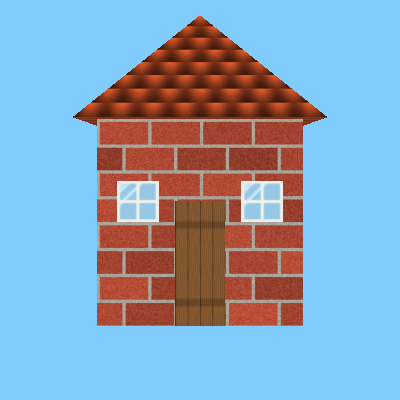
\includegraphics[width=0.45\textwidth]{images/casa_frente.png}
    \caption{Casa vista de frente ($\theta_x = 0^\circ$, $\theta_y = 0^\circ$).}
    \label{fig:frente}
\end{figure}

A Figura~\ref{fig:poses} mostra a casa na pose inicial e depois de segurar as setas por alguns quadros. Como cada quadro gira $2^\circ$, segurar uma seta por 45 quadros gira a casa $90^\circ$.

\begin{itemize}
    \item \textbf{(a) Pose inicial:} a casa aparece vista de cima e um pouco de lado. À esquerda está a face frontal, com a porta e as duas janelas; à direita, a parede lateral direita com a sua janela; e em cima, o telhado, com duas faces e a aresta que sobe até o ápice;
    \item \textbf{(b) Seta para a direita:} depois de $90^\circ$ em $Y$, a parede lateral esquerda passou para a frente, com a sua única janela, e a face com a porta virou para o lado direito, aparecendo quase de perfil. O telhado continua igual, pois a pirâmide é simétrica;
    \item \textbf{(c) Seta para cima:} a casa tombou para trás e passou a ser vista por baixo. A maior face visível é o chão do corpo, que também tem a textura de tijolos, e por trás dele aparece o beiral do telhado. A parede lateral esquerda aparece no alto, de ponta-cabeça;
    \item \textbf{(d) Seta para baixo:} a casa tombou para o outro lado e o telhado passou a ser visto por cima, ocupando quase toda a imagem. As fileiras de telhas mudam de direção nas arestas que descem do ápice, mostrando onde termina uma face e começa a outra. Acima do telhado aparece a parede lateral esquerda, com a sua janela.
\end{itemize}

Em todas as poses, as partes escondidas foram corretamente encobertas: as janelas da parede oposta nunca aparecem através do corpo, e o telhado cobre o topo das paredes. Isso confirma que o Z-Buffer está funcionando com vários objetos desenhados em chamadas separadas. Também não houve \textit{z-fighting} entre as paredes e a porta ou as janelas.

\begin{figure}[H]
    \centering
    \begin{subfigure}[b]{0.24\textwidth}
        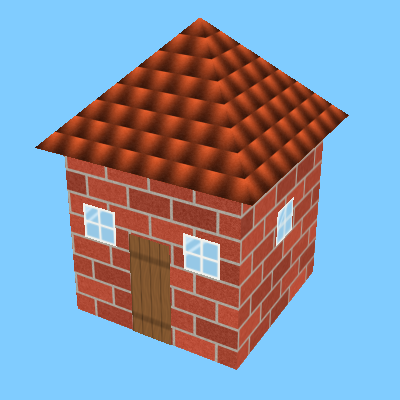
\includegraphics[width=\textwidth]{images/casa_inicial.png}
        \caption{$\theta_x = 25^\circ$, $\theta_y = -30^\circ$}
    \end{subfigure}
    \hfill
    \begin{subfigure}[b]{0.24\textwidth}
        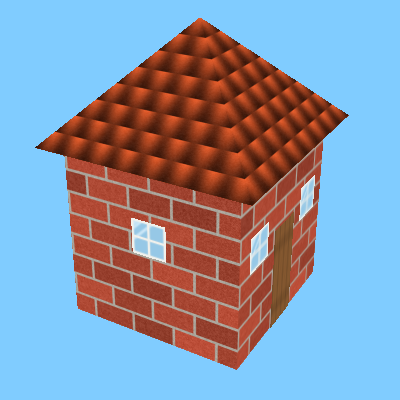
\includegraphics[width=\textwidth]{images/casa_direita.png}
        \caption{$\theta_x = 25^\circ$, $\theta_y = 60^\circ$}
    \end{subfigure}
    \hfill
    \begin{subfigure}[b]{0.24\textwidth}
        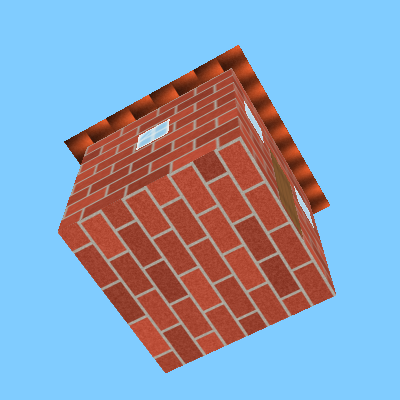
\includegraphics[width=\textwidth]{images/casa_cima.png}
        \caption{$\theta_x = -65^\circ$, $\theta_y = 60^\circ$}
    \end{subfigure}
    \hfill
    \begin{subfigure}[b]{0.24\textwidth}
        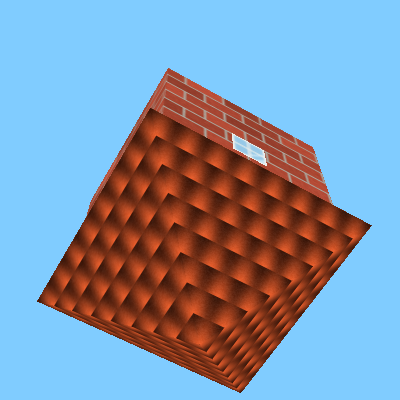
\includegraphics[width=\textwidth]{images/casa_baixo.png}
        \caption{$\theta_x = 115^\circ$, $\theta_y = 60^\circ$}
    \end{subfigure}
    \caption{Casa: (a) pose inicial; (b) após 45 quadros com a seta para a direita; (c) após mais 45 quadros com a seta para cima; (d) após mais 90 quadros com a seta para baixo.}
    \label{fig:poses}
\end{figure}

\subsection{Efeito dos Filtros de Textura}\label{sec:efeito_filtros}

Para mostrar na prática o que foi visto na Seção~\ref{sec:filtros}, o programa foi executado mais quatro vezes, trocando apenas os filtros e a posição da câmera, sem alterar o restante do código.

Na Figura~\ref{fig:mag}, a câmera foi colocada a apenas $0{,}1$ unidade da parede da frente, perto do canto de um tijolo. Nessa distância, cada texel da textura de tijolos ocupa cerca de 28 pixels na tela, e o filtro de ampliação é usado. Com \texttt{GL\_NEAREST} (a), cada texel vira um quadrado de cor única, e o ruído da textura aparece como um mosaico. Com \texttt{GL\_LINEAR} (b), usado no programa, as cores são misturadas pela Equação~\ref{eq:bilinear}, e a transição entre o tijolo e o rejunte fica suave.

\begin{figure}[H]
    \centering
    \begin{subfigure}[b]{0.45\textwidth}
        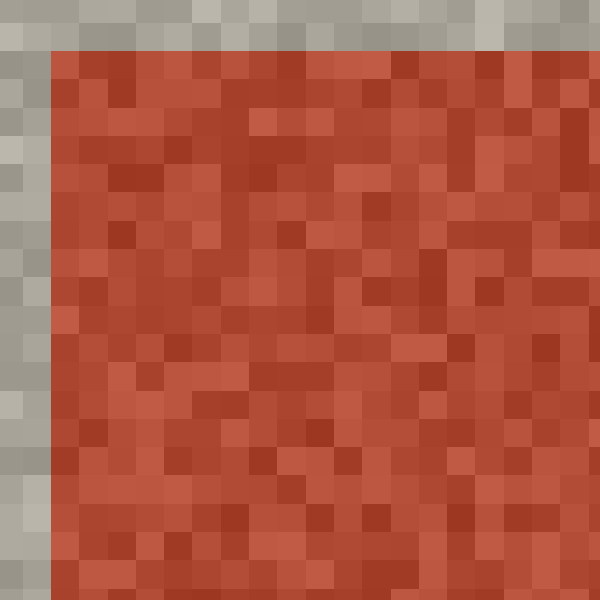
\includegraphics[width=\textwidth]{images/filtro_mag_nearest.png}
        \caption{\texttt{GL\_NEAREST}}
    \end{subfigure}
    \hfill
    \begin{subfigure}[b]{0.45\textwidth}
        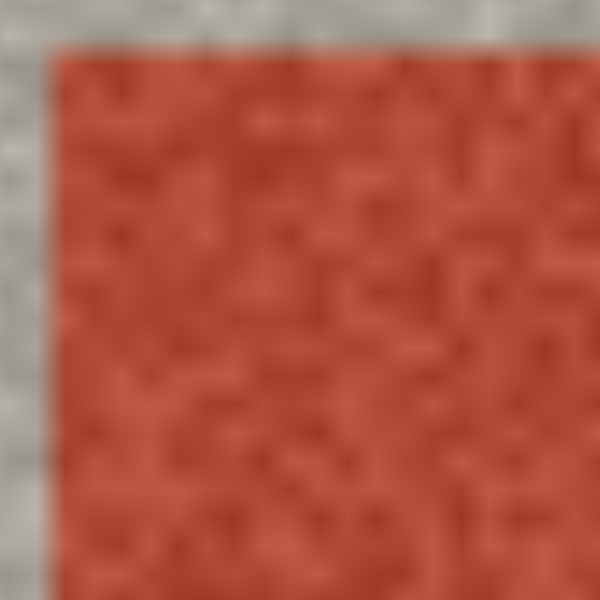
\includegraphics[width=\textwidth]{images/filtro_mag_linear.png}
        \caption{\texttt{GL\_LINEAR}}
    \end{subfigure}
    \caption{Ampliação: canto de um tijolo visto muito de perto com os dois filtros de ampliação.}
    \label{fig:mag}
\end{figure}

Na Figura~\ref{fig:min}, a câmera foi afastada para 30 unidades, e a casa passou a ocupar só cerca de 30 pixels de largura. Agora cada pixel cobre vários texels, e o filtro de redução é usado. A região ao redor da casa foi ampliada 5 vezes, sem interpolação, para que os pixels fiquem visíveis. Com \texttt{GL\_NEAREST} (a), cada pixel pega a cor de um único texel, escolhido praticamente ao acaso: as paredes ficam cheias de pontos cinza do rejunte espalhados sem padrão, as janelas viram listras e as telhas ficam salpicadas. Quando a casa gira, esses pontos mudam a cada quadro, gerando o ``serrilhado piscante'' citado em aula. Com o filtro trilinear e \textit{mipmaps} (b), usado no programa, a GPU lê os níveis pequenos, que já guardam a cor média de cada região. As paredes ficam com um vermelho uniforme, as janelas e a porta aparecem como manchas da sua cor real e a imagem não pisca durante o giro.

\begin{figure}[H]
    \centering
    \begin{subfigure}[b]{0.45\textwidth}
        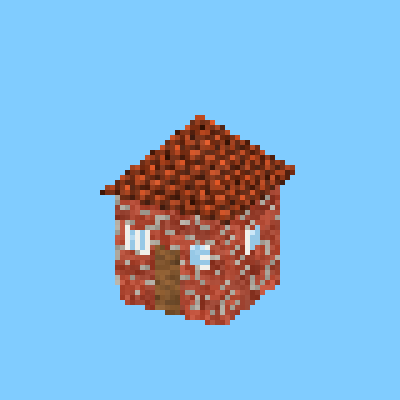
\includegraphics[width=\textwidth]{images/filtro_min_nearest.png}
        \caption{\texttt{GL\_NEAREST}}
    \end{subfigure}
    \hfill
    \begin{subfigure}[b]{0.45\textwidth}
        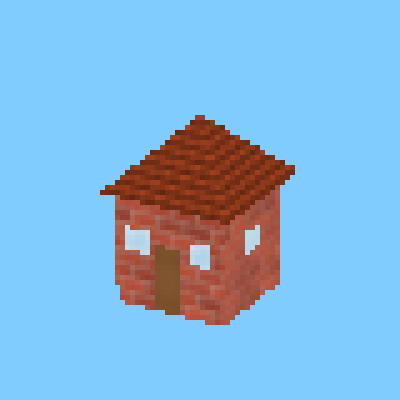
\includegraphics[width=\textwidth]{images/filtro_min_mipmap.png}
        \caption{\texttt{GL\_LINEAR\_MIPMAP\_LINEAR}}
    \end{subfigure}
    \caption{Redução: casa vista de longe (30 unidades) com os dois filtros de redução. Imagens ampliadas 5 vezes.}
    \label{fig:min}
\end{figure}

\subsection{Conferência da Matriz MVP}

Para conferir as contas, a matriz MVP da pose inicial ($\theta_x = 25^\circ$, $\theta_y = -30^\circ$) foi calculada com as mesmas funções do programa:

\begin{equation}
MVP = \begin{bmatrix}
1{,}5681  & 0         & -0{,}9053 & 0 \\
-0{,}5101 & 2{,}188   & -0{,}8836 & -0{,}7243 \\
-0{,}4541 & -0{,}4235 & -0{,}7865 & 3{,}8078 \\
-0{,}4532 & -0{,}4226 & -0{,}7849 & 4
\end{bmatrix}
\end{equation}

Aplicando essa matriz ao ápice do telhado, $[0;\ 1{,}1;\ 0;\ 1]^T$, obtém-se $[0;\ 1{,}6826;\ 3{,}342;\ 3{,}5351]^T$. Dividindo por $w = 3{,}5351$, o ápice vai para $x = 0$ e $y = 0{,}476$ na tela normalizada. Convertendo para a janela de $800\times600$, isso corresponde ao pixel $(400;\ 157)$. Na imagem capturada, o pixel mais alto da casa está em $(398;\ 158)$, ou seja, a menos de 2 pixels do valor calculado, uma diferença que vem do arredondamento feito pelo rasterizador e da suavização das bordas do telhado.

\section{Conclusão}

A atividade mostrou que a textura dá muito mais detalhe a um sólido sem aumentar a quantidade de vértices. A casa inteira tem apenas 60 vértices e 28 triângulos, mas os tijolos, as telhas, as tábuas da porta e as vidraças aparecem com riqueza de detalhes, porque esse detalhe está nas imagens, e não na geometria. A estrutura do programa (janela, contexto, matrizes, \textit{shaders} e laço principal) foi reaproveitada do cubo da aula. As mudanças foram a função \texttt{criar\_vao}, para não repetir o mesmo bloco quatro vezes, e a troca da textura ligada ao slot 0 antes de desenhar cada objeto.

Também ficou claro o papel da interpolação em duas etapas diferentes. Primeiro, o rasterizador interpola as coordenadas UV entre os vértices, para que cada pixel saiba onde ler na imagem. Depois, o filtro de textura interpola as cores entre os texels vizinhos. As comparações da Seção~\ref{sec:efeito_filtros} mostraram que, sem essa segunda interpolação, a textura fica pixelada de perto e cheia de \textit{aliasing} de longe, e que os \textit{mipmaps}, com apenas um terço a mais de memória, resolvem o problema da redução. Por fim, detalhes como a inversão vertical da imagem, a ordem das UVs em cada face e o pequeno deslocamento da porta e das janelas para evitar o \textit{z-fighting} mostraram que mapear texturas exige atenção à forma como o OpenGL enxerga as coordenadas.

\begin{thebibliography}{9}

\bibitem{rodrigo_textura}
RODRIGO, Raulivan. \textbf{Shaders: Interpolação de Textura}. Notas de Aula (17 - Shaders - Interpolação de Textura.pdf). Departamento de Computação, Centro Federal de Educação Tecnológica de Minas Gerais (CEFET-MG), 2026.

\bibitem{rodrigo_shaders}
RODRIGO, Raulivan. \textbf{Shaders}. Notas de Aula (16 - Shaders.pdf). Departamento de Computação, Centro Federal de Educação Tecnológica de Minas Gerais (CEFET-MG), 2026.

\bibitem{rodrigo_glfw}
RODRIGO, Raulivan. \textbf{GLFW - Graphics Library Framework}. Notas de Aula (15 - GLFW - Graphics Library Framework.pdf). Departamento de Computação, Centro Federal de Educação Tecnológica de Minas Gerais (CEFET-MG), 2026.

\bibitem{rodrigo_cubo_textura}
RODRIGO, Raulivan. \textbf{cubo\_textura.py}. Repositório computacao-grafica-python. Disponível em: \url{https://github.com/raulivan/computacao-grafica-python/blob/main/AULA17/cubo_textura.py}.

\bibitem{khronos_texparameter}
KHRONOS GROUP. \textbf{glTexParameter - OpenGL 4 Reference Pages}. Disponível em: \url{https://registry.khronos.org/OpenGL-Refpages/gl4/html/glTexParameter.xhtml}.

\bibitem{glfw_docs}
GLFW DEVELOPMENT TEAM. \textbf{GLFW Documentation}. Disponível em: \url{https://www.glfw.org/documentation.html}.

\bibitem{pyopengl_docs}
PYOPENGL DEVELOPERS. \textbf{PyOpenGL Documentation}. Disponível em: \url{https://pyopengl.sourceforge.net/documentation/}.

\bibitem{pillow_docs}
PILLOW CONTRIBUTORS. \textbf{Pillow Documentation}. Disponível em: \url{https://pillow.readthedocs.io/}.

\bibitem{numpy_docs}
NUMPY DEVELOPERS. \textbf{NumPy Documentation}. Disponível em: \url{https://numpy.org/doc/stable/}.

\end{thebibliography}

\end{document}
